\documentclass[]{article}
\usepackage{lmodern}
\usepackage{amssymb,amsmath}
\usepackage{ifxetex,ifluatex}
\usepackage{fixltx2e} % provides \textsubscript
\ifnum 0\ifxetex 1\fi\ifluatex 1\fi=0 % if pdftex
  \usepackage[T1]{fontenc}
  \usepackage[utf8]{inputenc}
\else % if luatex or xelatex
  \ifxetex
    \usepackage{mathspec}
  \else
    \usepackage{fontspec}
  \fi
  \defaultfontfeatures{Ligatures=TeX,Scale=MatchLowercase}
\fi
% use upquote if available, for straight quotes in verbatim environments
\IfFileExists{upquote.sty}{\usepackage{upquote}}{}
% use microtype if available
\IfFileExists{microtype.sty}{%
\usepackage[]{microtype}
\UseMicrotypeSet[protrusion]{basicmath} % disable protrusion for tt fonts
}{}
\PassOptionsToPackage{hyphens}{url} % url is loaded by hyperref
\usepackage[unicode=true]{hyperref}
\hypersetup{
            pdftitle={BRUV data summary 2019},
            pdfauthor={Jessica Madden},
            pdfborder={0 0 0},
            breaklinks=true}
\urlstyle{same}  % don't use monospace font for urls
\usepackage[margin=1in]{geometry}
\usepackage{graphicx,grffile}
\makeatletter
\def\maxwidth{\ifdim\Gin@nat@width>\linewidth\linewidth\else\Gin@nat@width\fi}
\def\maxheight{\ifdim\Gin@nat@height>\textheight\textheight\else\Gin@nat@height\fi}
\makeatother
% Scale images if necessary, so that they will not overflow the page
% margins by default, and it is still possible to overwrite the defaults
% using explicit options in \includegraphics[width, height, ...]{}
\setkeys{Gin}{width=\maxwidth,height=\maxheight,keepaspectratio}
\IfFileExists{parskip.sty}{%
\usepackage{parskip}
}{% else
\setlength{\parindent}{0pt}
\setlength{\parskip}{6pt plus 2pt minus 1pt}
}
\setlength{\emergencystretch}{3em}  % prevent overfull lines
\providecommand{\tightlist}{%
  \setlength{\itemsep}{0pt}\setlength{\parskip}{0pt}}
\setcounter{secnumdepth}{0}
% Redefines (sub)paragraphs to behave more like sections
\ifx\paragraph\undefined\else
\let\oldparagraph\paragraph
\renewcommand{\paragraph}[1]{\oldparagraph{#1}\mbox{}}
\fi
\ifx\subparagraph\undefined\else
\let\oldsubparagraph\subparagraph
\renewcommand{\subparagraph}[1]{\oldsubparagraph{#1}\mbox{}}
\fi

% set default figure placement to htbp
\makeatletter
\def\fps@figure{htbp}
\makeatother

\usepackage{booktabs}
\usepackage{longtable}
\usepackage{array}
\usepackage{multirow}
\usepackage{wrapfig}
\usepackage{float}
\usepackage{colortbl}
\usepackage{pdflscape}
\usepackage{tabu}
\usepackage{threeparttable}
\usepackage{threeparttablex}
\usepackage[normalem]{ulem}
\usepackage{makecell}

\title{BRUV data summary 2019}
\author{Jessica Madden}
\date{November 30, 2020}

\begin{document}
\maketitle

A total of \textbf{39 species} belonging to \textbf{17 families} were
recorded from BRUV deployments at all of the locations combined. This
summary includes MaxN data recorded to species (with the exception of
the category `unknown silversides'). There are a number of point tags
that are to genus, family, or unknown that are not included here, though
these tags that are excluded should not greatly affect the species
richness or MaxN data represented here.

\subsubsection{Species Richness}\label{species-richness}

\emph{\textbf{Table 1.} Total species richness at each site. Species
richness represents number of unique species (Actinopterygii,
Elasmobranchii) observed in all BRUV videos at each site (n = 9). For
all MPA/Reference pairs except the San Diego site, the MPA site had
greater species richness.}

\begin{table}[H]
\centering
\begin{tabular}[t]{l|l|r}
\hline
Site & Type & Species richness\\
\hline
Percos & MPA & 12\\
\hline
Refugio & Reference & 11\\
\hline
South Campus & MPA & 19\\
\hline
Haskells & Reference & 12\\
\hline
Dume Cove & MPA & 18\\
\hline
Leo Carrillo & Reference & 12\\
\hline
Sleepy Hollow & MPA & 22\\
\hline
Strands & Reference & 14\\
\hline
Scripps & MPA & 12\\
\hline
San Elijo & Reference & 15\\
\hline
\end{tabular}
\end{table}

\includegraphics{bruv-data-summary_files/figure-latex/unnamed-chunk-5-1.pdf}

\emph{\textbf{Figure 1.} Total species richness at each site. Species
richness represents number of unique species (Actinopterygii,
Elasmobranchii) observed in all BRUV videos at each site (n = 9). Sites
are ordered MPA first and reference second, with pairs in order of
decreasing latitude.}

\subsubsection{Mean Species Richness}\label{mean-species-richness}

\emph{\textbf{Table 2.} Summary statistics of species richness from BRUV
deployments at ten sampling locations. Mean species richness represents
the number of unique species (Actinopterygii, Elasmobranchii) observed
in each deployment averaged across all deployments for each site.}

\begin{table}[H]
\centering
\begin{tabular}{l|l|r|r|r|r|r|r}
\hline
Site & Type & Mean species richness & SD & Min & Max & Median & n\\
\hline
Percos & MPA & 3.78 & 1.56 & 2 & 6 & 4 & 9\\
\hline
Refugio & Reference & 3.89 & 1.45 & 2 & 7 & 4 & 9\\
\hline
South Campus & MPA & 7.22 & 2.82 & 3 & 11 & 8 & 9\\
\hline
Haskells & Reference & 3.67 & 1.12 & 2 & 5 & 4 & 9\\
\hline
Dume Cove & MPA & 6.56 & 1.33 & 5 & 9 & 6 & 9\\
\hline
Leo Carrillo & Reference & 4.78 & 1.56 & 2 & 7 & 5 & 9\\
\hline
Sleepy Hollow & MPA & 5.67 & 3.20 & 1 & 13 & 5 & 9\\
\hline
Strands & Reference & 4.67 & 2.65 & 1 & 8 & 4 & 9\\
\hline
Scripps & MPA & 5.11 & 1.83 & 2 & 8 & 5 & 9\\
\hline
San Elijo & Reference & 4.56 & 1.81 & 2 & 8 & 5 & 9\\
\hline
\end{tabular}
\end{table}

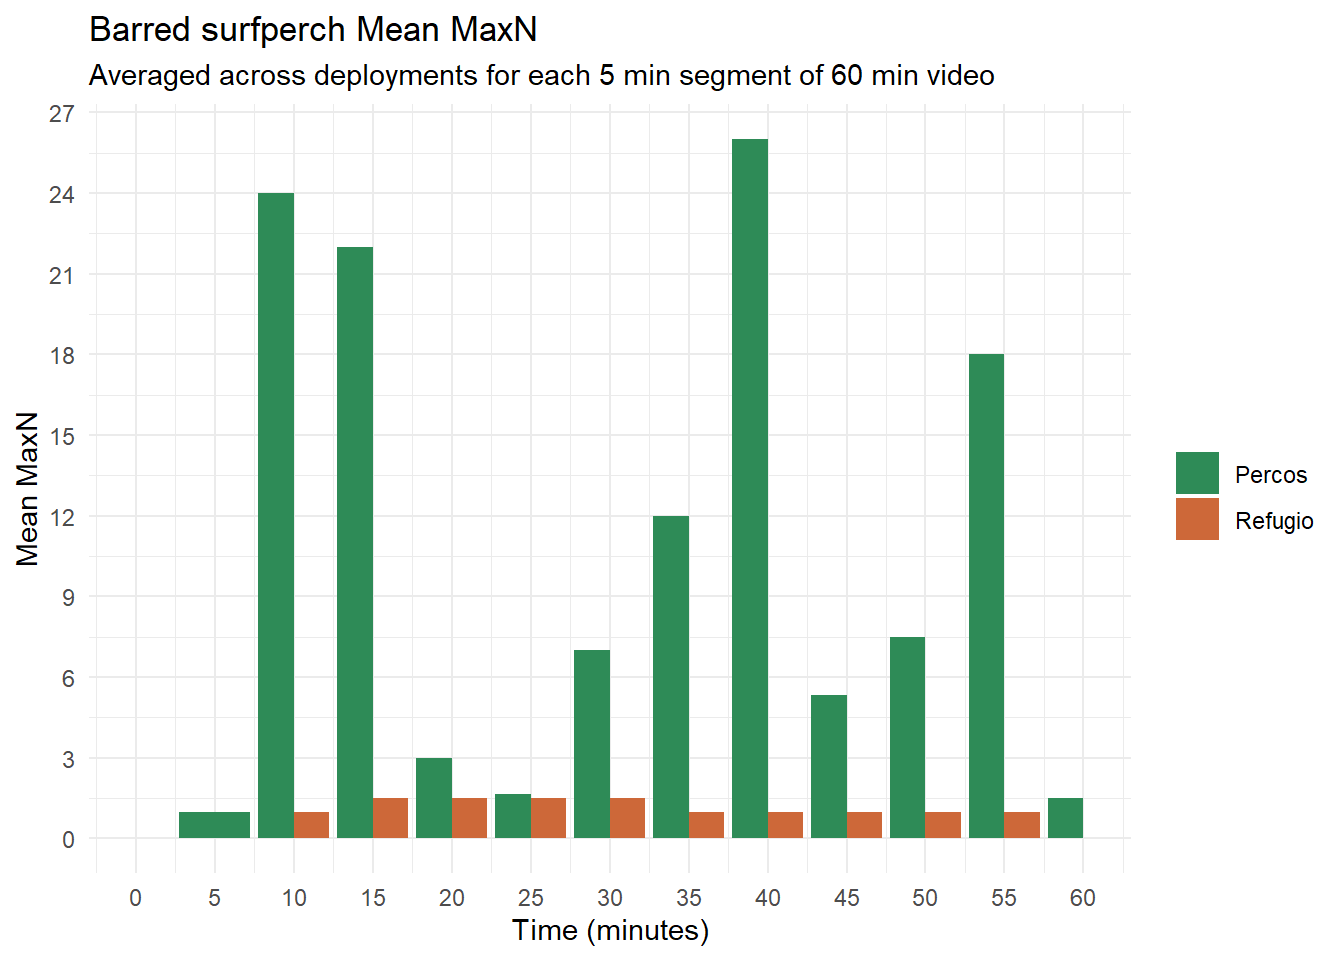
\includegraphics{bruv-data-summary_files/figure-latex/unnamed-chunk-8-1.pdf}

\emph{\textbf{Figure 2.} Mean species richness at each site. Mean
species richness represents the number of unique species
(Actinopterygii, Elasmobranchii) observed in each deployment averaged
across all deployments for each site (n = 9). Error bars indicate
standard deviation from the mean. Sites are ordered MPA first and
reference second, with pairs in order of decreasing latitude.}

\subsubsection{Mean species ricness:
Actinopterygii}\label{mean-species-ricness-actinopterygii}

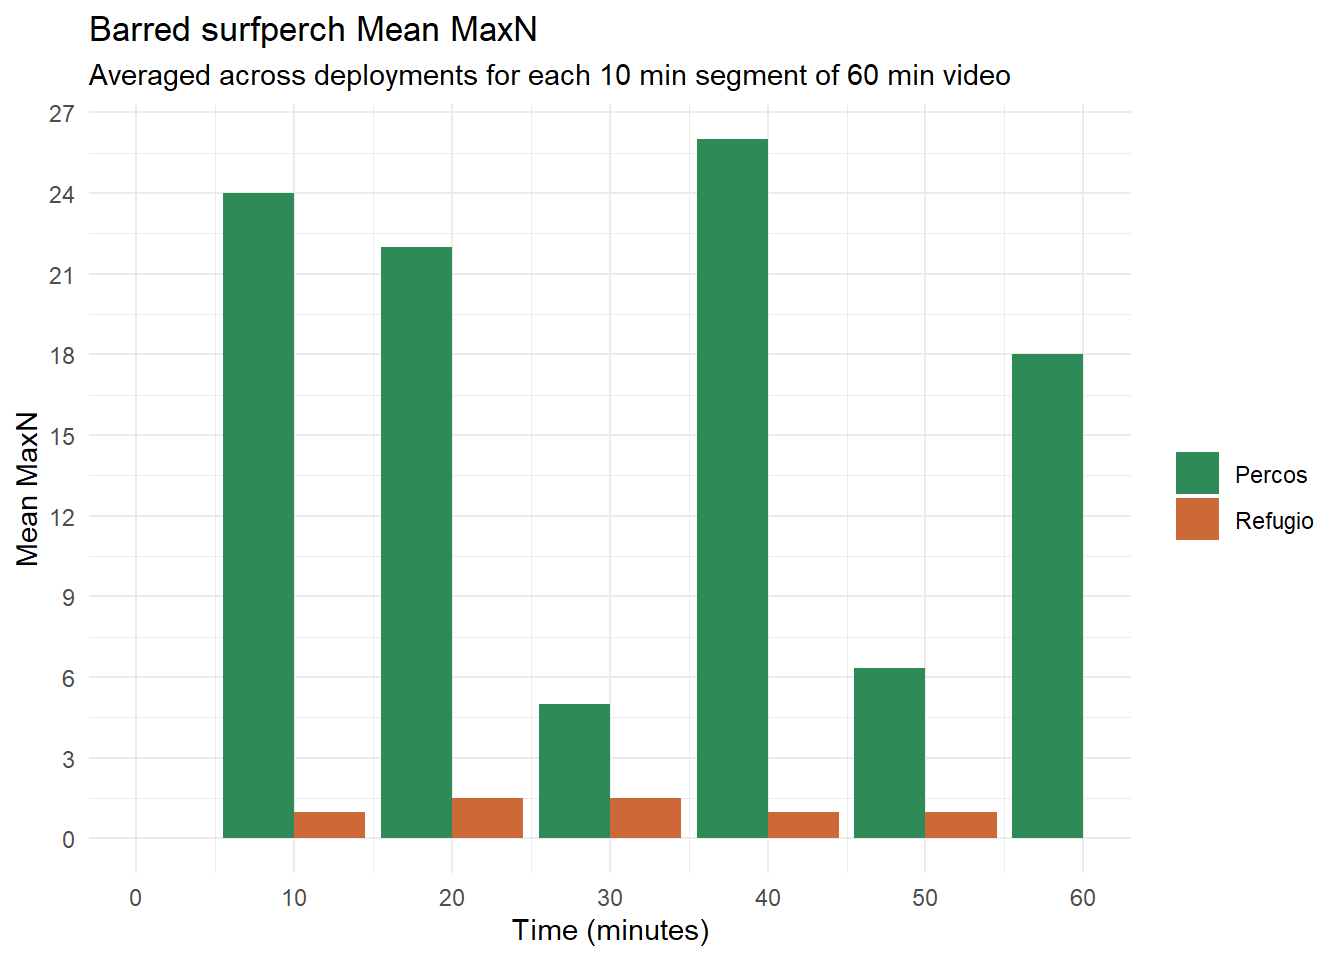
\includegraphics{bruv-data-summary_files/figure-latex/unnamed-chunk-9-1.pdf}

\subsubsection{Mean species ricness:
Elasmobranchii}\label{mean-species-ricness-elasmobranchii}

\includegraphics{bruv-data-summary_files/figure-latex/unnamed-chunk-10-1.pdf}

\subsubsection{MaxN}\label{maxn}

\paragraph{MaxN by species}\label{maxn-by-species}

MaxN statistic represents the maximum number of individuals belonging to
each species counted in a single frame, across all sampling videos at
each site (n = 9). Max \% presence is the percentage of deployments in
which a species is present, from the site in which the species had the
highest \% presence.

\emph{\textbf{Table 3.} MaxN statistic for each species present at the
10 sampling locations and Max \% presence at any one location. }

\begin{table}[H]
\centering
\begin{tabular}{l|l|r|r|r|r|r|r|r|r|r|r|r}
\hline
Common name & Family & Max \% presence & Percos & Refugio & South Campus & Haskells & Dume Cove & Leo Carrillo & Sleepy Hollow & Strands & Scripps & San Elijo\\
\hline
Topsmelt & Atherinopsidae & 56 & 4 & 5 &  & 20 & 28 & 3 &  & 1 & 99 & \\
\hline
Unknown Silverside & Atherinopsidae & 56 &  & 2 & 40 & 12 & 129 & 1 & 1 & 14 & 158 & 103\\
\hline
Pacific jack mackerel & Carangidae & 11 &  &  &  & 3 &  &  &  &  &  & \\
\hline
Diamond stingray & Dasyatidae & 22 &  &  &  &  &  &  &  &  & 1 & \\
\hline
Black perch & Embiotocidae & 44 &  &  & 3 &  & 9 &  & 1 &  &  & \\
\hline
Pile perch & Embiotocidae & 11 &  &  &  &  & 1 &  &  &  &  & \\
\hline
Walleye surfperch & Embiotocidae & 33 & 145 & 10 & 2 &  & 26 & 17 &  &  &  & 4\\
\hline
Barred surfperch & Embiotocidae & 67 & 46 & 2 & 3 & 8 &  & 5 &  &  &  & \\
\hline
Calico surfperch & Embiotocidae & 11 & 2 &  &  &  &  &  &  &  &  & \\
\hline
Shiner perch & Embiotocidae & 11 &  & 1 &  &  &  &  &  &  &  & \\
\hline
Silver surfperch & Embiotocidae & 11 &  & 18 &  &  &  &  &  &  &  & \\
\hline
Dwarf perch & Embiotocidae & 56 &  &  & 3 &  &  &  &  &  &  & \\
\hline
Rainbow surfperch & Embiotocidae & 11 &  &  & 1 &  &  &  &  &  &  & \\
\hline
Rubberlip seaperch & Embiotocidae & 11 &  &  & 1 &  &  &  &  &  &  & \\
\hline
Sargo & Haemulidae & 56 &  &  & 1 &  & 2 &  & 1 &  & 1 & 1\\
\hline
Horn shark & Heterodontidae & 22 &  &  & 1 &  &  & 1 &  &  &  & \\
\hline
Halfmoon & Kyphosidae & 33 &  &  &  &  & 1 &  & 2 &  &  & \\
\hline
Opaleye & Kyphosidae & 22 &  &  &  &  & 2 &  & 1 & 3 &  & \\
\hline
Zebra perch & Kyphosidae & 56 &  &  &  &  & 32 &  & 1 & 6 &  & \\
\hline
California sheephead & Labridae & 44 &  &  &  &  & 3 &  & 1 & 1 &  & \\
\hline
Rock wrasse & Labridae & 22 &  &  & 1 &  & 1 &  & 2 &  &  & 1\\
\hline
California moray & Muraenidae & 22 &  &  &  &  &  &  & 1 &  &  & \\
\hline
Bat ray & Myliobatidae & 89 & 1 & 1 & 2 & 1 & 2 & 1 & 1 & 1 & 4 & 2\\
\hline
Speckled sanddab & Paralichthyidae & 89 & 7 & 6 &  & 3 & 1 &  & 1 &  & 1 & \\
\hline
California halibut & Paralichthyidae & 11 & 1 & 1 &  &  &  &  &  &  &  & \\
\hline
Pacific sanddab & Paralichthyidae & 22 & 1 &  &  &  &  &  & 1 &  &  & \\
\hline
Thornback guitarfish & Platyrhinidae & 56 & 2 & 2 & 2 & 1 & 1 & 1 & 1 &  & 1 & 1\\
\hline
Shovelnose guitarfish & Rhinobatidae & 78 & 2 & 1 & 2 & 1 & 1 & 1 & 2 &  & 1 & 1\\
\hline
Yellowfin croaker & Sciaenidae & 67 &  &  & 1 & 1 & 5 & 5 & 130 & 5 & 3 & 73\\
\hline
California corbina & Sciaenidae & 44 & 5 &  &  & 1 &  & 1 & 2 & 1 & 2 & 2\\
\hline
Queenfish & Sciaenidae & 11 &  &  &  &  &  &  & 92 &  &  & 60\\
\hline
Spotfin croaker & Sciaenidae & 22 &  &  &  &  &  &  & 11 & 4 &  & 1\\
\hline
Black croaker & Sciaenidae & 22 &  &  & 1 &  &  &  &  &  &  & \\
\hline
White seabass & Sciaenidae & 11 &  &  &  &  &  &  &  & 1 &  & \\
\hline
Kelp bass & Serranidae & 100 &  &  & 3 &  & 6 &  & 12 & 6 &  & \\
\hline
Barred sand bass & Serranidae & 44 &  &  & 1 &  &  &  & 2 & 2 &  & 1\\
\hline
Leopard shark & Triakidae & 100 & 1 &  & 7 & 1 & 2 & 2 & 1 & 4 & 1 & 1\\
\hline
Grey smooth-hound & Triakidae & 11 &  &  &  &  &  &  &  &  &  & 1\\
\hline
Round stingray & Urotrygonidae & 89 &  &  & 1 & 1 &  & 1 & 2 & 1 & 6 & 1\\
\hline
\end{tabular}
\end{table}

\includegraphics{bruv-data-summary_files/figure-latex/unnamed-chunk-13-1.pdf}

\emph{\textbf{Figure 3.} MaxN statistic for each site. Sites are ordered
MPA first and reference second, with pairs in order of decreasing
latitude. Stacked colors indicate unique species, with the exception of
`unknown silversides' possibly including topsmelt.}

\includegraphics{bruv-data-summary_files/figure-latex/unnamed-chunk-14-1.pdf}

\emph{\textbf{Figure 4.} Composition of species at each site as a
proportion of MaxN recorded. Sites are ordered MPA first and reference
second, with pairs in order of decreasing latitude. Stacked colors
indicate unique species, with the exception of `unknown silversides'
possibly including topsmelt.}

\paragraph{Max N by family}\label{max-n-by-family}

\includegraphics{bruv-data-summary_files/figure-latex/unnamed-chunk-15-1.pdf}

\emph{\textbf{Figure 5. } MaxN statistic agregated by family for each
site. Sites are ordered MPA first and reference second, with pairs in
order of decreasing latitude. Stacked colors indicate unique families.}

\includegraphics{bruv-data-summary_files/figure-latex/unnamed-chunk-16-1.pdf}

\emph{\textbf{Figure 6.} Composition of species aggregated by family at
each site as a proportion of MaxN recorded. Percent contribution of MAxN
is between 0 - 1.0. Sites are ordered MPA first and reference second,
with pairs in order of decreasing latitude. Stacked colors indicate
unique families.}

\paragraph{Mean maxN}\label{mean-maxn}

\emph{\textbf{Table 3.} Summary statistics of average maxN of species at
each site out of n deployments. This average includes maxN = 0 for
deployments in which a species known to be present at the site is
absent.}

\begin{table}[H]
\centering
\begin{tabular}{l|l|r|r|r|r|r|r|r|r|r|r|r|r|r|r|r|r|r|r|r|r}
\hline
Common name & Family & Percos Mean MaxN & Percos SD & Refugio Mean MaxN & Refugio SD & South Campus Mean MaxN & South Campus SD & Haskells Mean MaxN & Haskells SD & Dume Cove Mean MaxN & Dume Cove SD & Leo Carrillo Mean MaxN & Leo Carrillo SD & Sleepy Hollow Mean MaxN & Sleepy Hollow SD & Strands Mean MaxN & Strands SD & Scripps Mean MaxN & Scripps SD & San Elijo Mean MaxN & San Elijo SD\\
\hline
Topsmelt & Atherinopsidae & 1.00 & 1.58 & 2.00 & 2.35 &  &  & 4.33 & 6.71 & 3.11 & 9.33 & 0.67 & 1.32 &  &  & 0.11 & 0.33 & 11.00 & 33.00 &  & \\
\hline
Unknown Silverside & Atherinopsidae &  &  & 0.89 & 0.93 & 4.56 & 13.30 & 1.67 & 3.94 & 23.00 & 43.43 & 0.44 & 0.53 & 0.11 & 0.33 & 2.00 & 4.69 & 26.78 & 51.21 & 19.00 & 34.89\\
\hline
Pacific jack mackerel & Carangidae &  &  &  &  &  &  & 0.33 & 1.00 &  &  &  &  &  &  &  &  &  &  &  & \\
\hline
Diamond stingray & Dasyatidae &  &  &  &  &  &  &  &  &  &  &  &  &  &  &  &  & 0.22 & 0.44 &  & \\
\hline
Barred surfperch & Embiotocidae & 7.22 & 15.08 & 0.44 & 0.73 & 1.11 & 1.05 & 1.11 & 2.67 &  &  & 1.56 & 1.81 &  &  &  &  &  &  &  & \\
\hline
Calico surfperch & Embiotocidae & 0.22 & 0.67 &  &  &  &  &  &  &  &  &  &  &  &  &  &  &  &  &  & \\
\hline
Walleye surfperch & Embiotocidae & 16.11 & 48.33 & 1.22 & 3.31 & 0.44 & 0.73 &  &  & 4.22 & 9.08 & 2.00 & 5.63 &  &  &  &  &  &  & 0.44 & 1.33\\
\hline
Shiner perch & Embiotocidae &  &  & 0.11 & 0.33 &  &  &  &  &  &  &  &  &  &  &  &  &  &  &  & \\
\hline
Silver surfperch & Embiotocidae &  &  & 2.00 & 6.00 &  &  &  &  &  &  &  &  &  &  &  &  &  &  &  & \\
\hline
Black perch & Embiotocidae &  &  &  &  & 0.89 & 1.17 &  &  & 1.33 & 3.04 &  &  & 0.11 & 0.33 &  &  &  &  &  & \\
\hline
Dwarf perch & Embiotocidae &  &  &  &  & 0.78 & 0.97 &  &  &  &  &  &  &  &  &  &  &  &  &  & \\
\hline
Rainbow surfperch & Embiotocidae &  &  &  &  & 0.11 & 0.33 &  &  &  &  &  &  &  &  &  &  &  &  &  & \\
\hline
Rubberlip seaperch & Embiotocidae &  &  &  &  & 0.11 & 0.33 &  &  &  &  &  &  &  &  &  &  &  &  &  & \\
\hline
Pile perch & Embiotocidae &  &  &  &  &  &  &  &  & 0.11 & 0.33 &  &  &  &  &  &  &  &  &  & \\
\hline
Sargo & Haemulidae &  &  &  &  & 0.33 & 0.50 &  &  & 0.67 & 0.71 &  &  & 0.11 & 0.33 &  &  & 0.11 & 0.33 & 0.11 & 0.33\\
\hline
Horn shark & Heterodontidae &  &  &  &  & 0.11 & 0.33 &  &  &  &  & 0.22 & 0.44 &  &  &  &  &  &  &  & \\
\hline
Halfmoon & Kyphosidae &  &  &  &  &  &  &  &  & 0.33 & 0.50 &  &  & 0.22 & 0.67 &  &  &  &  &  & \\
\hline
Opaleye & Kyphosidae &  &  &  &  &  &  &  &  & 0.22 & 0.67 &  &  & 0.11 & 0.33 & 0.44 & 1.01 &  &  &  & \\
\hline
Zebra perch & Kyphosidae &  &  &  &  &  &  &  &  & 6.89 & 11.05 &  &  & 0.22 & 0.44 & 1.11 & 1.96 &  &  &  & \\
\hline
Rock wrasse & Labridae &  &  &  &  & 0.11 & 0.33 &  &  & 0.11 & 0.33 &  &  & 0.33 & 0.71 &  &  &  &  & 0.11 & 0.33\\
\hline
California sheephead & Labridae &  &  &  &  &  &  &  &  & 0.67 & 1.00 &  &  & 0.22 & 0.44 & 0.33 & 0.50 &  &  &  & \\
\hline
California moray & Muraenidae &  &  &  &  &  &  &  &  &  &  &  &  & 0.22 & 0.44 &  &  &  &  &  & \\
\hline
Bat ray & Myliobatidae & 0.33 & 0.50 & 0.11 & 0.33 & 0.67 & 0.87 & 0.56 & 0.53 & 0.78 & 0.67 & 0.56 & 0.53 & 0.33 & 0.50 & 0.33 & 0.50 & 1.89 & 1.27 & 0.67 & 0.71\\
\hline
California halibut & Paralichthyidae & 0.11 & 0.33 & 0.11 & 0.33 &  &  &  &  &  &  &  &  &  &  &  &  &  &  &  & \\
\hline
Pacific sanddab & Paralichthyidae & 0.11 & 0.33 &  &  &  &  &  &  &  &  &  &  & 0.22 & 0.44 &  &  &  &  &  & \\
\hline
Speckled sanddab & Paralichthyidae & 3.78 & 2.44 & 1.78 & 1.72 &  &  & 0.56 & 1.13 & 0.11 & 0.33 &  &  & 0.11 & 0.33 &  &  & 0.11 & 0.33 &  & \\
\hline
Thornback guitarfish & Platyrhinidae & 0.67 & 0.87 & 0.78 & 0.83 & 0.44 & 0.73 & 0.11 & 0.33 & 0.11 & 0.33 & 0.56 & 0.53 & 0.33 & 0.50 &  &  & 0.33 & 0.50 & 0.22 & 0.44\\
\hline
Shovelnose guitarfish & Rhinobatidae & 0.78 & 0.83 & 0.33 & 0.50 & 1.00 & 0.71 & 0.33 & 0.50 & 0.22 & 0.44 & 0.22 & 0.44 & 0.44 & 0.73 &  &  & 0.56 & 0.53 & 0.44 & 0.53\\
\hline
California corbina & Sciaenidae & 0.56 & 1.67 &  &  &  &  & 0.11 & 0.33 &  &  & 0.22 & 0.44 & 0.44 & 0.73 & 0.22 & 0.44 & 0.56 & 0.73 & 0.33 & 0.71\\
\hline
Black croaker & Sciaenidae &  &  &  &  & 0.22 & 0.44 &  &  &  &  &  &  &  &  &  &  &  &  &  & \\
\hline
Yellowfin croaker & Sciaenidae &  &  &  &  & 0.11 & 0.33 & 0.22 & 0.44 & 0.89 & 1.62 & 1.44 & 1.67 & 20.11 & 44.39 & 0.56 & 1.67 & 0.78 & 1.09 & 13.22 & 24.23\\
\hline
Queenfish & Sciaenidae &  &  &  &  &  &  &  &  &  &  &  &  & 10.22 & 30.67 &  &  &  &  & 6.67 & 20.00\\
\hline
Spotfin croaker & Sciaenidae &  &  &  &  &  &  &  &  &  &  &  &  & 1.67 & 3.74 & 0.56 & 1.33 &  &  & 0.22 & 0.44\\
\hline
White seabass & Sciaenidae &  &  &  &  &  &  &  &  &  &  &  &  &  &  & 0.11 & 0.33 &  &  &  & \\
\hline
Barred sand bass & Serranidae &  &  &  &  & 0.11 & 0.33 &  &  &  &  &  &  & 0.44 & 0.73 & 0.44 & 0.73 &  &  & 0.11 & 0.33\\
\hline
Kelp bass & Serranidae &  &  &  &  & 1.22 & 0.83 &  &  & 2.44 & 1.81 &  &  & 3.89 & 4.86 & 1.78 & 2.11 &  &  &  & \\
\hline
Leopard shark & Triakidae & 0.22 & 0.44 &  &  & 2.78 & 1.86 & 0.67 & 0.50 & 1.22 & 0.83 & 0.67 & 0.71 & 0.22 & 0.44 & 1.56 & 1.13 & 0.44 & 0.53 & 0.67 & 0.50\\
\hline
Grey smooth-hound & Triakidae &  &  &  &  &  &  &  &  &  &  &  &  &  &  &  &  &  &  & 0.11 & 0.33\\
\hline
Round stingray & Urotrygonidae &  &  &  &  & 0.33 & 0.50 & 0.22 & 0.44 &  &  & 0.33 & 0.50 & 0.89 & 0.60 & 0.44 & 0.53 & 2.44 & 1.74 & 0.56 & 0.53\\
\hline
\end{tabular}
\end{table}

\textbf{(a)}
\includegraphics{bruv-data-summary_files/figure-latex/unnamed-chunk-20-1.pdf}

\textbf{(b)}
\includegraphics{bruv-data-summary_files/figure-latex/unnamed-chunk-21-1.pdf}

\textbf{(c)}
\includegraphics{bruv-data-summary_files/figure-latex/unnamed-chunk-22-1.pdf}

\textbf{(d)}
\includegraphics{bruv-data-summary_files/figure-latex/unnamed-chunk-23-1.pdf}

\textbf{(e)}
\includegraphics{bruv-data-summary_files/figure-latex/unnamed-chunk-24-1.pdf}

\emph{\textbf{Figure 7 (a-e).} Average MaxN of all species observed at
each site for each site pair. Error bars were left off because of
relatively large standard deviation (see Table 3). }

Pull species list from maxN data

\end{document}
